\chapter{PAPER-128}
\label{c.PSA128}

\section{Overview}

The PAPER experiment expanded out to 128 antennas in 2013 and observed for two seasons. The first season began in November, 2013 and lasted until March, 2014. The second began in July, 2014 and ended in January, 2015. The PAPER-128 configuration consists of 112 core antennas arranged in a grid layout (7 rows and 16 columns), with neighboring East/West spacings being 15\,m and neighboring North/South spacings being 4\,m (Figure \ref{fig:paper128_array}). Additionally, 16 outrigger antennas are placed in strategic locations in order to form long baselines and increase \textit{uv}-plane sampling. These outrigger antennas are not used for the power spectrum analysis presented in this thesis, but are useful for imaging analyses.

\begin{figure}
	\centering
	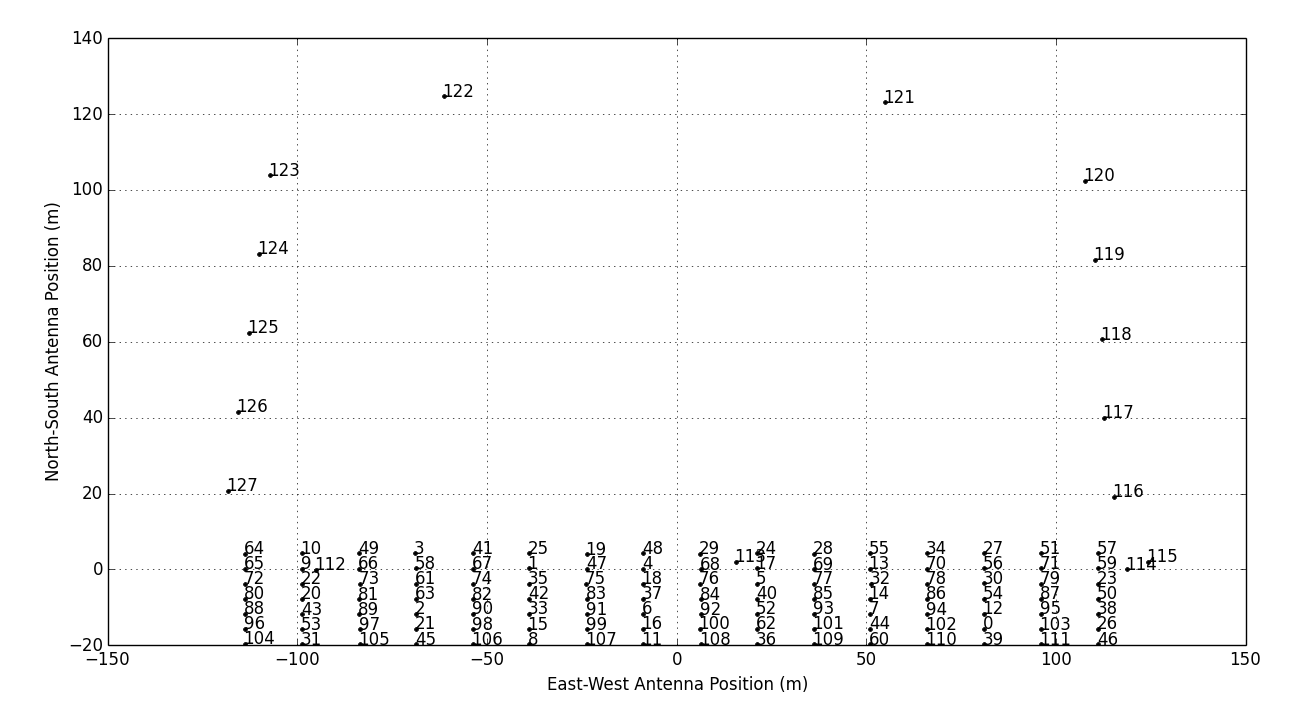
\includegraphics[width=0.96\textwidth]{plots/paper128_layout.png}
	\caption{The PAPER-128 antenna layout. There are 112 antennas arranged in a grid layout which are used for power spectrum analyses. The addition of 16 outrigger antennas is used to increase \textit{uv}-plane sampling for imaging analyses.}
	\label{fig:paper128_array}
\end{figure}

In general, the signal chain of PAPER-128 is similar to that of PAPER-64. However, one major change is the addition of receiverators on site, which houses the receivers used to amplify and filter the antenna signals. Prior to this change, the receivers were located inside a cooled shipping container along with the rest of the DSP system. With the addition of more antennas, however, the receivers were moved outside the container to save space. 

Although PAPER-128 doubled in the number of antennas, the data collected by this array is typically found to be lower in quality than that of PAPER-64. There are many reasons for this, including general wear and tear on the instrument and the addition of the receiverators (which had no monitoring system and, as we will see, is one of the main reasons for missing and corrupted PAPER-128 data). Because of these issues, PAPER-128 requires the development of novel techniques in order to filter out contaminated data products prior to analysis. Using the entire season of data, without any filtering, would result in a power spectrum analysis dominated by systematics and (non-EoR) detections. Thus, one of the unique challenges facing PAPER-128 is how to automatically and accurately detect and remove bad data (i.e., misbehaving baselines, dead receiverators, criss-crossed signal paths, etc.) in order to curate a dataset as free of systematics as possible.

In this chapter, we present methods developed for the detection of corrupt data in PAPER-128. These methods represent the first routinely-used ``quality assurance" steps for the PAPER experiment. They also represent the first generation of data assessment techniques, which are currently being expanded upon for incorporation into HERA's real-time processing system. 

Additionally, we process two epochs of PAPER-128 data (both from the first season) and show power spectrum results for each. We do not show the second season of data due to increased hardware failure that was experienced at the end of PAPER-128's run. As such, the first season of PAPER-128 represents the bulk of the array's sensitivity (though we note that the limits do not surpass those of PAPER-64, mostly due to having fewer days of data).

\section{Quality Assurance}
\subsection{Flagging Julian Dates}
\subsection{Flagging Antennas}
\section{Data Processing}
\section{Power Spectrum Limits}




